\documentclass{article}


\usepackage{arxiv}
\usepackage{amsmath}
\usepackage[utf8]{inputenc} % allow utf-8 input
\usepackage[T1]{fontenc}    % use 8-bit T1 fonts
\usepackage{xr-hyper}       % cross-references to the main article
\usepackage{hyperref}       % hyperlinks
\usepackage{url}            % simple URL typesetting
\usepackage{booktabs}       % professional-quality tables
\usepackage{amsfonts}       % blackboard math symbols
\usepackage{nicefrac}       % compact symbols for 1/2, etc.
\usepackage{microtype}      % microtypography
\usepackage{lipsum}
\usepackage{graphicx}
\usepackage{amssymb}
\usepackage{natbib}

\graphicspath{ {./images/} }
\externaldocument{modularity}


\title{Supplemental Information for\\Sparsity-driven Emergence of Functional Modularity in Multitask Neural Networks}


\author{Bowen Shi$^{1,2}$ \quad Qi Ouyang$^{1,3,4}$ \quad Long Qian$^{2,3}$\\
\small $^1$Institute for Advanced Study in Physics, Zhejiang University, Hangzhou 310058, China\\
\small $^2$Center for Quantitative Biology, Academy for Advanced Interdisciplinary Studies,\\
\small Peking University, Beijing 100871, China\\
\small $^3$ZJU--Hangzhou Global Scientific and Technological Innovation Center, Hangzhou 311200, China\\
\small $^4$Institute of Fundamental and Transdisciplinary Research, Zhejiang University, Hangzhou, China\\
\texttt{sbw1996@zju.edu.cn; qoy@zju.edu.cn; longqian@pku.edu.cn}
}
  %% \AND
  %% Coauthor \\
  %% Affiliation \\
  %% Address \\
  %% \texttt{email} \\
  %% \And
  %% Coauthor \\
  %% Affiliation \\
  %% Address \\
  %% \texttt{email} \\
  %% \And
  %% Coauthor \\
  %% Affiliation \\
  %% Address \\
  %% \texttt{email} \\

\begin{document}
\maketitle

\setcounter{section}{0}
\setcounter{equation}{0}
\setcounter{figure}{0}
\setcounter{table}{0}
\renewcommand{\thesection}{S\arabic{section}}
\renewcommand{\thesubsection}{\thesection.\arabic{subsection}}
\renewcommand{\thesubsubsection}{\thesubsection.\arabic{subsubsection}}
\renewcommand{\theequation}{S.\arabic{equation}}
\renewcommand{\thefigure}{S\arabic{figure}}
\renewcommand{\thetable}{S\arabic{table}}

\section{A Local Support-Recovery Argument for \(L_\gamma\)-Induced Subnetworks}
\label{appendix:lgamma_subnetwork_recovery}
\label{appendix:proofLasso}

This supplemental section gives a conditional proof explaining why sparsity-inducing \(L_\gamma\) regularization can make task-selective functional-token subnetworks separable by ablation or Taylor profiling. The argument starts from the linear multitask model
\begin{equation}
Y=XB_0+E,
\label{eq:appendix_linear_model}
\end{equation}
and then transfers the conclusion to a trained neural network through an explicit local-linear surrogate assumption. It should be read as a support-recovery theorem for the surrogate coordinates, not as a global theorem for nonlinear training dynamics.

\subsection{Linear surrogate and notation}

Let \(n\) be the number of samples, \(p\) the number of candidate elementary coordinates, and \(R\) the number of tasks. In Eq.~\eqref{eq:appendix_linear_model},
\begin{equation}
X\in\mathbb R^{n\times p},\qquad
Y=[Y_1,\ldots,Y_R]\in\mathbb R^{n\times R},\qquad
B_0=[\beta_{0,1},\ldots,\beta_{0,R}]\in\mathbb R^{p\times R},
\end{equation}
where \(Y_r\in\mathbb R^n\) is the target vector for task \(r\), \(\beta_{0,r}\in\mathbb R^p\) is the true task-specific coefficient vector, and \(E=[\varepsilon_1,\ldots,\varepsilon_R]\) is the noise matrix. For each task,
\begin{equation}
Y_r=X\beta_{0,r}+\varepsilon_r .
\end{equation}
We write
\begin{equation}
C=\frac{1}{n}X^\top X,
\qquad
\mathcal S_r=\{j:\beta_{0,jr}\ne0\},
\qquad
\mathcal S_r^c=\{1,\ldots,p\}\setminus\mathcal S_r,
\qquad
s_r=|\mathcal S_r|.
\end{equation}
Here \(\mathcal S_r\) is the true support of task \(r\). To avoid confusing support sets with importance scores, this section uses calligraphic \(\mathcal S\) for supports and reserves symbols such as \(S^{\mathrm{abl}}_{r,q}\) and \(S^{\mathrm{tay}}_{r,q}\) for ablation and Taylor scores.

We estimate \(B_0\) by
\begin{equation}
\widehat B_\gamma\in
\arg\min_B
Q_\gamma(B),
\qquad
Q_\gamma(B)=
\frac{1}{2n}\|Y-XB\|_F^2+
\lambda\sum_{j=1}^{p}\sum_{r=1}^{R}|B_{jr}|^\gamma,
\qquad 0<\gamma\le1 .
\label{eq:lgamma_multitask_objective}
\end{equation}
The objective is separable across task columns:
\begin{equation}
Q_\gamma(B)=\sum_{r=1}^{R}q_{\gamma,r}(\beta_r),
\qquad
q_{\gamma,r}(\beta)=
\frac{1}{2n}\|Y_r-X\beta\|_2^2+
\lambda\sum_{j=1}^{p}|\beta_j|^\gamma .
\end{equation}
It is therefore enough to prove the support claim for one fixed task. In the proof below we suppress the task index \(r\), writing \(Y,\beta_0,\varepsilon,\mathcal S\) for the corresponding single-task quantities.

\subsection{Assumptions}

The following assumptions are standard support-recovery assumptions, with an additional local-curvature condition for the nonconvex case \(0<\gamma<1\).

\paragraph{A1. Sparse and normalized design.}
The support size satisfies \(s=|\mathcal S|\ll p\). The columns of \(X\) are normalized so that \(C_{jj}=1\), and \(\|C\|_{op}\le M_C\) for a finite constant \(M_C\). Here \(\|\cdot\|_{op}\) denotes the spectral norm.

\paragraph{A2. Restricted identifiability.}
There are constants \(m>0\) and \(M_S<\infty\) such that
\begin{equation}
\lambda_{\min}(C_{\mathcal S\mathcal S})\ge m,
\qquad
\|C_{\mathcal S\mathcal S}^{-1}\|_\infty\le M_S .
\label{eq:restricted_identifiability_lgamma}
\end{equation}
For index sets \(A,B\), \(C_{AB}\) denotes the submatrix of \(C\) with rows in \(A\) and columns in \(B\). The matrix \(\infty\)-norm is the maximum absolute row sum.

\paragraph{A3. Noise correlation.}
The empirical noise-design correlation is uniformly bounded:
\begin{equation}
\left\|\frac{1}{n}X^\top\varepsilon\right\|_\infty\le\tau_n .
\label{eq:noise_correlation_lgamma}
\end{equation}
For normalized designs and sub-Gaussian noise, \(\tau_n\) is typically of order \(\sqrt{\log p/n}\) for one task, or \(\sqrt{\log(pR)/n}\) uniformly across \(R\) tasks.

\paragraph{A4. Beta-min signal.}
The smallest active coefficient is bounded below:
\begin{equation}
b_{\min}=\min_{j\in\mathcal S}|\beta_{0,j}|>0 .
\end{equation}
The tuning parameter \(\lambda\) is small enough that active coefficients do not cross zero. A convenient sufficient condition is
\begin{equation}
M_S\{\tau_n+\lambda\gamma(b_{\min}/2)^{\gamma-1}\}<b_{\min}/2 .
\label{eq:beta_min_lgamma_subnetwork}
\end{equation}
For \(\gamma=1\), this is \(M_S(\tau_n+\lambda)<b_{\min}/2\).

\paragraph{A5. Off-support incoherence for \(\gamma=1\).}
For the Lasso endpoint, assume the strict irrepresentable condition
\begin{equation}
\left\|
C_{\mathcal S^c\mathcal S}C_{\mathcal S\mathcal S}^{-1}
\operatorname{sign}(\beta_{0,\mathcal S})
\right\|_\infty
\le1-\eta,
\qquad 0<\eta\le1,
\label{eq:irrepresentable_lgamma_subnetwork}
\end{equation}
and assume the off-support noise is dominated by the Lasso penalty:
\begin{equation}
\left(1+\left\|C_{\mathcal S^c\mathcal S}C_{\mathcal S\mathcal S}^{-1}\right\|_\infty\right)\tau_n
\le \eta\lambda .
\label{eq:lasso_noise_dominance_lgamma}
\end{equation}
These two inequalities are used only for the convex \(\gamma=1\) support-recovery proof.

\paragraph{A6. Active-set curvature for \(0<\gamma<1\).}
For \(0<\gamma<1\), \(|b|^\gamma\) is concave away from zero, so its second derivative is negative on active coordinates. We assume the restricted quadratic loss curvature dominates that negative curvature in the sign-preserving neighborhood \(|b_j|\ge b_{\min}/2\): there is \(\mu>0\) such that
\begin{equation}
\lambda_{\min}(C_{\mathcal S\mathcal S})
-
\lambda\gamma(1-\gamma)(b_{\min}/2)^{\gamma-2}
\ge \mu .
\label{eq:active_curvature_lgamma_subnetwork}
\end{equation}
In addition, the active gradient at the oracle coefficient is small enough that
\begin{equation}
\sqrt{s}\left\{\tau_n+\lambda\gamma(b_{\min}/2)^{\gamma-1}\right\}<\mu b_{\min}/4 .
\label{eq:nonconvex_boundary_lgamma}
\end{equation}
This condition ensures that the restricted nonconvex problem has an interior minimizer in the sign-preserving neighborhood.

\subsection{Support recovery for \(0<\gamma\le1\)}

\paragraph{Proposition S1.}
Under A1--A6, the following statements hold for each task \(r\).

For \(\gamma=1\), the convex Lasso problem has a global minimizer \(\widehat\beta_{1,r}\) satisfying
\begin{equation}
\operatorname{supp}(\widehat\beta_{1,r})=\mathcal S_r,
\qquad
\operatorname{sign}(\widehat\beta_{1,\mathcal S_r,r})=
\operatorname{sign}(\beta_{0,\mathcal S_r,r}).
\end{equation}

For \(0<\gamma<1\), the nonconvex objective has a strict local minimizer \(\widehat\beta_{\gamma,r}^{\mathrm{loc}}\) satisfying
\begin{equation}
\operatorname{supp}(\widehat\beta_{\gamma,r}^{\mathrm{loc}})=\mathcal S_r,
\qquad
\operatorname{sign}(\widehat\beta_{\gamma,\mathcal S_r,r}^{\mathrm{loc}})=
\operatorname{sign}(\beta_{0,\mathcal S_r,r}).
\end{equation}
The second statement is local: it does not claim that all global minimizers have this support, nor that gradient descent from arbitrary initialization must reach this local minimizer.

\paragraph{Proof.}
Fix a task and omit the subscript \(r\).

\emph{Case 1: \(\gamma=1\).}
The objective is convex. We use a primal-dual witness argument. The phrase Karush-Kuhn-Tucker (KKT) conditions refers here to the necessary and sufficient first-order optimality conditions for a convex optimization problem with a nonsmooth penalty, expressed through the subgradient of the \(\ell_1\) norm.

First solve the restricted Lasso problem on the true support:
\begin{equation}
\widehat\beta_{\mathcal S}
\in
\arg\min_{b\in\mathbb R^s}
\left\{
\frac{1}{2n}\|Y-X_{\mathcal S}b\|_2^2+
\lambda\|b\|_1
\right\},
\qquad
\widehat\beta_{\mathcal S^c}=0 .
\end{equation}
On active coordinates, the KKT equation is
\begin{equation}
C_{\mathcal S\mathcal S}(\widehat\beta_{\mathcal S}-\beta_{0,\mathcal S})
-
\frac{1}{n}X_{\mathcal S}^\top\varepsilon
+
\lambda z_{\mathcal S}=0,
\label{eq:kkt_active_lasso_lgamma}
\end{equation}
where \(z_{\mathcal S}\in\partial\|\widehat\beta_{\mathcal S}\|_1\). If \(\widehat\beta_{\mathcal S}\) has the correct sign, then \(z_{\mathcal S}=\operatorname{sign}(\beta_{0,\mathcal S})\). Solving Eq.~\eqref{eq:kkt_active_lasso_lgamma} gives
\begin{equation}
\widehat\beta_{\mathcal S}-\beta_{0,\mathcal S}
=
C_{\mathcal S\mathcal S}^{-1}
\left(
\frac{1}{n}X_{\mathcal S}^\top\varepsilon-
\lambda z_{\mathcal S}
\right).
\end{equation}
By A2--A4 with \(\gamma=1\),
\begin{equation}
\|\widehat\beta_{\mathcal S}-\beta_{0,\mathcal S}\|_\infty
\le M_S(\tau_n+\lambda)<b_{\min}/2 .
\end{equation}
Thus every active coefficient remains nonzero and has the same sign as \(\beta_{0,\mathcal S}\). This validates the chosen active subgradient.

It remains to verify the inactive KKT condition. For \(j\in\mathcal S^c\), the subgradient condition for \(\widehat\beta_j=0\) is
\begin{equation}
\left\|
C_{\mathcal S^c\mathcal S}(\widehat\beta_{\mathcal S}-\beta_{0,\mathcal S})
-
\frac{1}{n}X_{\mathcal S^c}^\top\varepsilon
\right\|_\infty
\le\lambda .
\label{eq:kkt_inactive_lasso_lgamma}
\end{equation}
Substituting the active solution with \(z_{\mathcal S}=\operatorname{sign}(\beta_{0,\mathcal S})\), the left side of Eq.~\eqref{eq:kkt_inactive_lasso_lgamma} is at most
\begin{equation}
\lambda
\left\|
C_{\mathcal S^c\mathcal S}C_{\mathcal S\mathcal S}^{-1}
\operatorname{sign}(\beta_{0,\mathcal S})
\right\|_\infty
+
\left(1+
\left\|C_{\mathcal S^c\mathcal S}C_{\mathcal S\mathcal S}^{-1}\right\|_\infty
\right)\tau_n .
\end{equation}
By A5 this is bounded by \(\lambda(1-\eta)+\eta\lambda=\lambda\). Therefore the full vector \((\widehat\beta_{\mathcal S},0)\) satisfies the KKT conditions. Since the \(\gamma=1\) objective is convex, these conditions certify a global minimizer with support \(\mathcal S\) and correct signs.

\emph{Case 2: \(0<\gamma<1\).}
The penalty is nonconvex and non-Lipschitz at zero, so KKT conditions at zero are not the right tool. We instead prove the existence of an oracle-supported strict local minimizer.

Consider the restricted objective on the true support:
\begin{equation}
q_{\gamma,\mathcal S}(b)=
\frac{1}{2n}\|Y-X_{\mathcal S}b\|_2^2+
\lambda\sum_{j\in\mathcal S}|b_j|^\gamma .
\end{equation}
Define the sign-preserving neighborhood
\begin{equation}
\mathcal N_{\mathcal S}=\{b:\|b-\beta_{0,\mathcal S}\|_\infty\le b_{\min}/2\}.
\end{equation}
Inside this neighborhood all active coordinates satisfy \(|b_j|\ge b_{\min}/2\). For any point in \(\mathcal N_{\mathcal S}\), the Hessian of the restricted objective is
\begin{equation}
\nabla^2 q_{\gamma,\mathcal S}(b)
=
C_{\mathcal S\mathcal S}
-
\lambda\gamma(1-\gamma)
\operatorname{diag}(|b_j|^{\gamma-2}:j\in\mathcal S),
\end{equation}
which is bounded below by \(\mu I\) by A6. Hence \(q_{\gamma,\mathcal S}\) is \(\mu\)-strongly convex on \(\mathcal N_{\mathcal S}\), even though the full objective is nonconvex outside this neighborhood.

At the oracle coefficient,
\begin{equation}
g_0=
\nabla q_{\gamma,\mathcal S}(\beta_{0,\mathcal S})
=
-
\frac{1}{n}X_{\mathcal S}^\top\varepsilon
+
\lambda\gamma|\beta_{0,\mathcal S}|^{\gamma-1}
\operatorname{sign}(\beta_{0,\mathcal S}).
\end{equation}
By A3 and A6,
\begin{equation}
\|g_0\|_2
\le
\sqrt{s}\{\tau_n+\lambda\gamma(b_{\min}/2)^{\gamma-1}\}
<\mu b_{\min}/4 .
\end{equation}
For any boundary point \(b=\beta_{0,\mathcal S}+u\) of \(\mathcal N_{\mathcal S}\), \(\|u\|_2\ge b_{\min}/2\). Strong convexity gives
\begin{equation}
q_{\gamma,\mathcal S}(\beta_{0,\mathcal S}+u)-q_{\gamma,\mathcal S}(\beta_{0,\mathcal S})
\ge
u^\top g_0+\frac{\mu}{2}\|u\|_2^2
\ge
-\|u\|_2\|g_0\|_2+\frac{\mu}{2}\|u\|_2^2>0 .
\end{equation}
Therefore the minimizer of \(q_{\gamma,\mathcal S}\) over the compact set \(\mathcal N_{\mathcal S}\) lies in its interior. Denote it by \(\widehat\beta_{\mathcal S}\). It satisfies the active first-order equation
\begin{equation}
C_{\mathcal S\mathcal S}(\widehat\beta_{\mathcal S}-\beta_{0,\mathcal S})
-
\frac{1}{n}X_{\mathcal S}^\top\varepsilon
+
\lambda\gamma|\widehat\beta_{\mathcal S}|^{\gamma-1}
\operatorname{sign}(\widehat\beta_{\mathcal S})=0 .
\label{eq:active_nonconvex_lgamma}
\end{equation}
Because \(\widehat\beta_{\mathcal S}\in\mathcal N_{\mathcal S}\), all active signs are preserved.

We now show that \((\widehat\beta_{\mathcal S},0)\) is a strict local minimizer in the full \(p\)-dimensional space. Perturb the active and inactive coordinates by \(u\in\mathbb R^s\) and \(v\in\mathbb R^{p-s}\), respectively. A Taylor expansion around \((\widehat\beta_{\mathcal S},0)\), using Eq.~\eqref{eq:active_nonconvex_lgamma} for the active coordinates, yields
\begin{align}
\Delta q(u,v)
&=
q_\gamma(\widehat\beta_{\mathcal S}+u,v)-q_\gamma(\widehat\beta_{\mathcal S},0) \\
&\ge
\frac{\mu}{2}\|u\|_2^2
+
 u^\top C_{\mathcal S\mathcal S^c}v
+
 a^\top v
-
\frac{M_C}{2}\|v\|_2^2
+
\lambda\sum_{j\in\mathcal S^c}|v_j|^\gamma,
\label{eq:delta_full_nonconvex_lgamma}
\end{align}
where
\begin{equation}
a=
C_{\mathcal S^c\mathcal S}(\widehat\beta_{\mathcal S}-\beta_{0,\mathcal S})
-
\frac{1}{n}X_{\mathcal S^c}^\top\varepsilon
\end{equation}
is finite by A1--A4. For \(0<\gamma<1\), the term \(\sum_j|v_j|^\gamma\) dominates both \(\|v\|_1\) and \(\|v\|_2^2\) as \(\|v\|_\infty\to0\): for sufficiently small \(\|v\|_\infty\),
\begin{equation}
\|v\|_1\le \|v\|_\infty^{1-\gamma}\sum_j|v_j|^\gamma,
\qquad
\|v\|_2^2\le \|v\|_\infty^{2-\gamma}\sum_j|v_j|^\gamma .
\end{equation}
The cross term satisfies, for any \(\alpha>0\),
\begin{equation}
|u^\top C_{\mathcal S\mathcal S^c}v|
\le
\alpha\|u\|_2^2+
\frac{\|C_{\mathcal S\mathcal S^c}\|_{op}^2}{4\alpha}\|v\|_2^2 .
\end{equation}
Choose \(\alpha<\mu/4\), then choose the neighborhood in \(v\) small enough that the inactive singular penalty dominates the finite linear term \(a^\top v\), the quadratic term in \(v\), and the remaining cross-term bound. Eq.~\eqref{eq:delta_full_nonconvex_lgamma} is then strictly positive for every nonzero sufficiently small perturbation \((u,v)\). Thus \((\widehat\beta_{\mathcal S},0)\) is a strict local minimizer with support \(\mathcal S\). This proves the nonconvex local statement.

Repeating the single-task argument for each task column proves the multitask statement, because Eq.~\eqref{eq:lgamma_multitask_objective} separates across tasks.

\subsection{From support recovery to score-separable functional tokens}

Support recovery says that the effective coordinates of task \(r\) form a set \(\mathcal S_r\). The experiments, however, do not observe \(\beta_{0,r}\) directly. They estimate functional supports through ablation and Taylor scores. This subsection proves the link between the true support \(\mathcal S_r\), the ablation score \(S^{\mathrm{abl}}_{r,q}\), and the Taylor score \(S^{\mathrm{tay}}_{r,q}\).

Let \(f_\theta\) be a trained network and fix a local coordinate block \(\ell\). Let \(z_q(x)\) denote the scalar local coordinate associated with weight token \(q\), for example the coordinate appearing in a parameter-Jacobian linearization around the trained parameters. Let \(f_r(x)\in\mathbb R^d\) be the output segment for task \(r\), where \(d=P\) in the experiments. Assume the following local-linear surrogate:
\begin{equation}
f_r(x)=\sum_{q=1}^{d_\ell}z_q(x)b_{qr}+\xi_r(x),
\qquad
b_{qr}\in\mathbb R^d,
\label{eq:local_linear_hidden_lgamma}
\end{equation}
where \(\xi_r(x)\) is a remainder term. The task support in this layer is
\begin{equation}
\mathcal S_{\ell,r}=\{q:\|b_{qr}\|_2>0\}.
\end{equation}
Define the ideal coefficient-energy score
\begin{equation}
G_{r,q}=\mathbb E\left[z_q(x)^2\right]\|b_{qr}\|_2^2 .
\label{eq:ideal_energy_score_lgamma}
\end{equation}
Assume an active margin: there exists \(\kappa>0\) such that
\begin{equation}
q\in\mathcal S_{\ell,r}\quad\Rightarrow\quad G_{r,q}\ge\kappa,
\qquad
q\notin\mathcal S_{\ell,r}\quad\Rightarrow\quad G_{r,q}=0 .
\label{eq:active_score_margin_lgamma}
\end{equation}
This margin excludes unidentifiable active coordinates with zero coordinate variance or vanishingly small effective coefficients.

\paragraph{Ablation score.}
Let \(f_r^{(-q)}(x)\) be the output after removing token \(q\). The population ablation score is
\begin{equation}
S^{\mathrm{abl}}_{r,q}=
\mathbb E\left\|f_r(x)-f_r^{(-q)}(x)\right\|_2^2 .
\label{eq:population_ablation_score_lgamma}
\end{equation}
If removing \(q\) changes only the corresponding local term up to a remainder
\begin{equation}
e^{\mathrm{abl}}_{r,q}(x)=
f_r(x)-f_r^{(-q)}(x)-z_q(x)b_{qr},
\qquad
\mathbb E\|e^{\mathrm{abl}}_{r,q}(x)\|_2^2\le \epsilon_{\mathrm{abl}}^2,
\end{equation}
and if \(G_{r,q}\le M_G\) uniformly, then
\begin{align}
\left|S^{\mathrm{abl}}_{r,q}-G_{r,q}\right|
&=
\left|\mathbb E\|z_qb_{qr}+e^{\mathrm{abl}}_{r,q}\|_2^2-
\mathbb E\|z_qb_{qr}\|_2^2\right| \\
&\le
2\sqrt{M_G}\epsilon_{\mathrm{abl}}+
\epsilon_{\mathrm{abl}}^2
=:\delta_{\mathrm{abl}} .
\label{eq:ablation_energy_bound_lgamma}
\end{align}
Thus ablation score is a controlled perturbation of the ideal support energy \(G_{r,q}\).

\paragraph{Taylor score.}
Introduce a multiplicative gate \(m_q\) on token \(q\), so that the local surrogate becomes
\begin{equation}
f_r(x;m)=\sum_{k=1}^{d_\ell}m_kz_k(x)b_{kr}+\xi_r(x;m),
\qquad m_k=1\ \text{at the trained network.}
\end{equation}
The population first-order Taylor score is
\begin{equation}
S^{\mathrm{tay}}_{r,q}=
\mathbb E\left\|
\left.
\frac{\partial f_r(x;m)}{\partial m_q}
\right|_{m=\mathbf 1}
\right\|_2^2 .
\label{eq:population_taylor_score_lgamma}
\end{equation}
Because
\begin{equation}
\left.
\frac{\partial f_r(x;m)}{\partial m_q}
\right|_{m=\mathbf 1}
=
z_q(x)b_{qr}+e^{\mathrm{tay}}_{r,q}(x),
\qquad
e^{\mathrm{tay}}_{r,q}(x)=
\left.
\frac{\partial \xi_r(x;m)}{\partial m_q}
\right|_{m=\mathbf 1},
\end{equation}
the same calculation gives, if \(\mathbb E\|e^{\mathrm{tay}}_{r,q}(x)\|_2^2\le\epsilon_{\mathrm{tay}}^2\),
\begin{equation}
\left|S^{\mathrm{tay}}_{r,q}-G_{r,q}\right|
\le
2\sqrt{M_G}\epsilon_{\mathrm{tay}}+
\epsilon_{\mathrm{tay}}^2
=:\delta_{\mathrm{tay}} .
\label{eq:taylor_energy_bound_lgamma}
\end{equation}

\paragraph{Score-support relation.}
Define score-threshold support estimates
\begin{equation}
\widehat{\mathcal S}^{\mathrm{abl}}_{\ell,r}(t)=
\{q:S^{\mathrm{abl}}_{r,q}>t\},
\qquad
\widehat{\mathcal S}^{\mathrm{tay}}_{\ell,r}(t)=
\{q:S^{\mathrm{tay}}_{r,q}>t\}.
\end{equation}
Let \(\delta=\max\{\delta_{\mathrm{abl}},\delta_{\mathrm{tay}}\}\). If \(\delta<\kappa/2\), then for every threshold
\begin{equation}
t\in(\delta,\kappa-\delta)
\end{equation}
we have
\begin{equation}
\widehat{\mathcal S}^{\mathrm{abl}}_{\ell,r}(t)
=
\widehat{\mathcal S}^{\mathrm{tay}}_{\ell,r}(t)
=
\mathcal S_{\ell,r}.
\label{eq:score_support_equivalence_lgamma}
\end{equation}
Indeed, if \(q\notin\mathcal S_{\ell,r}\), then \(G_{r,q}=0\), so both scores are at most \(\delta<t\). If \(q\in\mathcal S_{\ell,r}\), then \(G_{r,q}\ge\kappa\), so both scores are at least \(\kappa-\delta>t\). Moreover,
\begin{equation}
\left|S^{\mathrm{abl}}_{r,q}-S^{\mathrm{tay}}_{r,q}\right|
\le
\delta_{\mathrm{abl}}+\delta_{\mathrm{tay}},
\end{equation}
so ablation and Taylor are close because both estimate the same ideal energy \(G_{r,q}\), not because they are algebraically identical interventions.

The empirical scores have finite-sample error and, for Taylor profiling, random-probe error. If uniform bounds of sizes $c_N$ and $c_K$ hold for these two errors, the same conclusion holds after replacing $\delta$ by $\delta+c_N+c_K$. Four probes do not automatically guarantee the required bound; no numerical probe-error guarantee is asserted here. This is the formal relation between the recovered task support \(\mathcal S_{\ell,r}\), the ablation score \(S^{\mathrm{abl}}_{r,q}\), and the Taylor score \(S^{\mathrm{tay}}_{r,q}\).

\subsection{From linear supports to functional-token subnetworks}

The support-recovery result applies directly to coordinates on which the regularized objective acts, such as readout coefficients, explicit gates, path coefficients, or parameter-Jacobian coordinates. For scalar weight coordinates in a nonlinear network, raw sparsity must still be interpreted through a local surrogate. The bridge from Eq.~\eqref{eq:appendix_linear_model} to a neural network therefore requires a compatibility assumption: in the chosen local coordinates, the trained network is well approximated by Eq.~\eqref{eq:local_linear_hidden_lgamma}, and the effect of \(L_\gamma\) regularization is reflected in sparse, stable effective coefficients \(b_{qr}\) with a nonzero score margin \(\kappa\).

The support-recovery theorem and its singularity argument for $0<\gamma<1$ concern the idealized, unshifted penalty $|\beta|^\gamma$. The neural-network implementation instead uses $(|\theta|+10^{-8})^\gamma$ with per-matrix normalization (Section~\ref{appendix:architecture}). For this shifted penalty, the one-sided derivative has finite magnitude at zero; the unshifted singularity argument therefore does not directly prove local stability for the implemented objective. The theoretical connection remains conditional on the local-surrogate and compatibility assumptions above.

The support-recovery statement applies only when the realized score threshold, including the score floor, lies inside the assumed separation gap. A fixed 75th-percentile rule does not by itself guarantee this condition or identify the true support size. The theoretical noise bound $\tau_n$ is distinct from the extraction quantile $\tau=0.75$.

Under these local-surrogate, compatibility and score-separation assumptions, Proposition S1 yields task-specific supports \(\mathcal S_{\ell,r}\). Eq.~\eqref{eq:score_support_equivalence_lgamma} then shows that ablation and Taylor profiling recover those supports by thresholding. The task signature of token \(q\) is
\begin{equation}
\mathcal R_q=\{r:q\in\mathcal S_{\ell,r}\}.
\end{equation}
For a task set \(c\subseteq\{1,\ldots,R\}\), the retained functional-token subnetwork is the support union
\begin{equation}
U_c=\bigcup_{r\in c}\mathcal S_{\ell,r}
=\{q:\mathcal R_q\cap c\ne\varnothing\}.
\end{equation}
If \(r\in c\), then \(\mathcal S_{\ell,r}\subseteq U_c\). Provided the local approximation remains valid after the simultaneous mask is applied to all analyzed matrices, the surrogate gives
\begin{equation}
f_r^{(U_c)}(x)
\approx
\sum_{q\in \mathcal S_{\ell,r}}z_q(x)b_{qr}
\approx
f_r(x),
\end{equation}
which is a conditional output-preservation statement, not a general sufficiency guarantee for a nonlinear network. Simultaneous removal of many weights can change activations and invalidate a single-coordinate approximation. Preserving thresholded predictions additionally requires the joint-mask output error to remain smaller than the original distance of each output from its decision threshold (0.5 for binary outputs). Support inclusion alone does not establish this stability or margin condition. If \(s\notin c\), and the same approximation remains valid, then
\begin{equation}
f_s^{(U_c)}(x)
\approx
\sum_{q\in U_c\cap\mathcal S_{\ell,s}}z_q(x)b_{qs}.
\end{equation}
A small intersection \(U_c\cap\mathcal S_{\ell,s}\) alone does not imply reduced off-target accuracy: the magnitudes of omitted contributions, biases, approximation error and classification margins also matter. An accuracy decrease requires output changes that cross decision boundaries in directions that turn correct predictions into errors, with a net loss over any corrected errors. Sufficiency and specificity of the actual joint masks are therefore assessed empirically. Finally,
\begin{equation}
U_{c_1\cup c_2}=U_{c_1}\cup U_{c_2},
\end{equation}
which explains why functional-token combinations can be composed by union of their recovered supports. This is the mathematical counterpart of the experimental masking rule: retain scalar weight tokens important for any selected task and remove the rest.

\subsection{Why the endpoint \(\gamma=1\) is included and why \(\gamma>1\) differs}

The endpoint \(\gamma=1\) is included because the Lasso penalty has a subgradient interval at zero:
\begin{equation}
\partial |b|\big|_{b=0}=[-1,1].
\end{equation}
This interval is exactly what allows the inactive KKT condition in Eq.~\eqref{eq:kkt_inactive_lasso_lgamma} to hold with \(\widehat\beta_j=0\). Thus \(\gamma=1\) can produce exact zeros and support recovery under the irrepresentable and beta-min conditions above.

For \(0<\gamma<1\), the derivative
\begin{equation}
\frac{d}{db}|b|^\gamma=\gamma |b|^{\gamma-1}\operatorname{sign}(b),
\qquad b\ne0,
\end{equation}
is singular as \(b\to0\). This singularity makes zero locally stable against sufficiently small inactive perturbations, which is why the nonconvex proof uses local domination by \(\sum_j|v_j|^\gamma\) rather than a convex KKT certificate.

For \(\gamma>1\), neither mechanism is present. There is no Lasso subgradient interval at zero, and the derivative is finite at zero; for \(\gamma=2\), it is exactly zero at zero. Small empirical correlations can then be represented by small nonzero coefficients instead of being thresholded to exact zeros. Consequently, task supports need not have a stable active/inactive gap, and ablation or Taylor score distributions may not admit a clean threshold separating functional-token subnetworks.

\subsection{Conclusion of the argument}

Combining the pieces gives the conditional chain
\begin{equation}
\begin{aligned}
L_\gamma\ (0<\gamma\le1)
&\quad\Longrightarrow\quad
\text{support recovery in a compatible local surrogate}
\\[-1pt]
&\quad\Longrightarrow\quad
\mathcal S_{\ell,r}
\quad\Longrightarrow\quad
\widehat{\mathcal S}^{\mathrm{abl}}_{\ell,r}
=
\widehat{\mathcal S}^{\mathrm{tay}}_{\ell,r}
=
\mathcal S_{\ell,r},
\end{aligned}
\end{equation}
provided the restricted-design, beta-min, noise, curvature, local-linearization, and score-margin assumptions hold. This proves the claimed relationship between \(L_\gamma\)-induced sparse supports and threshold-separable ablation/Taylor functional-token subnetworks, while making explicit the assumptions under which the conclusion is valid.

\section{Model Architectures and Training Details}
\label{appendix:architecture}

\subsection{Multitask MLP}

The robustness simulations use a fully connected Torch MLP with three hidden layers, each containing 300 ReLU units. The input dimension is $d_{\mathrm{in}}=2P=14$ for the binary arithmetic and logic tasks, whereas paired MNIST images are flattened and concatenated to give $d_{\mathrm{in}}=2\times28\times28=1568$. The output dimension is $d_{\mathrm{out}}=RP$, with $R=5$ jointly trained rules and $P=7$ output bits per rule.

Each input sample contains two vectors, $\mathbf{x}$ and $\mathbf{y}$, concatenated into a shared input representation. The model is trained on rule indices 0--4, displayed in the paper as rules 1--5. Each rule defines a distinct transformation of the same input pair and produces an output vector of length $P$. The rule-specific outputs are concatenated and predicted by a shared network.

All tasks are introduced at the beginning of training and optimized jointly. We do not use curriculum learning, sequential task training, or task-specific pretraining. The training objective is
\[
\mathcal{L}=\frac{1}{R}\sum_{r=1}^{R}W_r\mathcal{L}_{r}+l_{\mathrm{train}}\Omega_\gamma(\theta),\qquad
\Omega_\gamma(\theta)=\sum_{B\in\mathcal{B}}\frac{1}{|B|}\sum_{q\in B}(|\theta_q|+\varepsilon)^\gamma,
\]
where $\mathcal{L}_{r}$ is the mean-squared error averaged over samples and the $P$ outputs of rule $r$, $W_r=1$ by default, $\mathcal{B}$ is the set of trainable non-bias weight matrices, and $|B|$ is the number of scalar weights in matrix $B$. The implementation uses $\varepsilon=10^{-8}$ and sums the per-matrix means rather than an unnormalized sum over all weights. Biases are excluded from the penalty. The task-weighting experiment sets one $W_r$ to 5 while retaining the factor $1/R$ and the same $l_{\mathrm{train}}$ (Supplementary Note~\ref{appendix:task_weighting_allocation}).

\paragraph{Robustness-simulation setup.}
\begin{itemize}
    \item Optimizer: Adam with learning rate $0.001$.
    \item Batch size: 128.
    \item Hidden layers: three layers with 300 units per layer.
    \item Dataset size: 5{,}000 samples with a 50/50 training--validation split.
    \item Independent repeats: 30, starting from seed 300.
    \item Number of jointly trained tasks: 5 in the default experiments.
    \item Regularization exponent: $\gamma=1$ in the robustness simulations; $\gamma\in\{0.5,1,2\}$ in the regularizer-form comparison.
    \item Sparsity coefficient: $l_1=5.0$ for MLP robustness simulations.
\end{itemize}

\paragraph{Training configurations by experiment.}
Saved training configurations distinguish the experiments listed below. All listed configurations use Adam, 5,000 training epochs, rules 1--5 (implementation indices 0--4), and a checkpoint interval of 1,000 epochs. Each experimental condition has 30 analyzed independent runs, except the TinyTransformer robustness analysis, which includes 23. The sweep contains 21 conditions; the task-weighting experiment contains six. The four mother-network conditions used for recomposition are drawn from the sweep and inherit its training settings.
\begin{center}
\small
\begin{tabular}{p{0.49\linewidth}rr}
\toprule
Experiment & Learning rate & Training batch size \\
\midrule
MLP robustness: binary, logic and MNIST & $10^{-3}$ & 128 \\
TinyTransformer robustness & $10^{-3}$ & 128 \\
Sparsity-strength/exponent sweep (Figs.~\ref{fig:main4}, \ref{fig:main5}) & $10^{-4}$ & 512 \\
Task weighting (Fig.~\ref{fig:main6}) & $5\times10^{-2}$ & 128 \\
Recomposition mother networks (Fig.~\ref{fig:main7}b,c) & $10^{-4}$ & 512 \\
\bottomrule
\end{tabular}
\end{center}
The TinyTransformer analysis uses the 23 saved runs trained with batch size 128. The seven runs trained with batch size 500 are excluded to keep the training batch size uniform; the original training records and analysis exports are retained. Training batch sizes in this table are distinct from the analysis batch size of 64 specified in the reproduction protocol. These values summarize saved configurations rather than software defaults; settings from one experiment are not transferred to another.

\subsection{TinyTransformer}

The TinyTransformer provides a lightweight non-MLP architecture for testing whether functional-token extraction depends on fully connected hidden layers. Each paired binary input is split into left and right halves, and both halves are projected into a shared 32-dimensional token space. The resulting two-token sequence is processed by two encoder-style self-attention blocks with feedforward width 64. The final representation is obtained by mean-pooling the two tokens and passing the pooled vector through a linear prediction head with $RP$ outputs.

In the robustness simulation, the TinyTransformer is trained on the same Binary Sequence Calculation rules as the MLP, using rule indices 0--4. The encoder is trainable (\texttt{train\_encoder=True}), so both the token encoder and output head are optimized jointly. Functional tokens are constructed from scalar weight coordinates in the trained parameter matrices, profiled and retained with the same definitions used for the MLP experiments.

\paragraph{Robustness-simulation setup.}
\begin{itemize}
    \item Optimizer: Adam with learning rate $0.001$.
    \item Training batch size: 128; 23 independent runs included in the analysis.
    \item Token/hidden dimension: 32.
    \item Transformer encoder blocks: two.
    \item Feedforward hidden dimension: 64.
    \item Dataset size: 5{,}000 binary-pair samples with a 50/50 training--validation split.
    \item Number of jointly trained arithmetic tasks: 5.
    \item Regularization exponent: $\gamma=1$.
    \item Sparsity coefficient: $l_1=0.5$ for the transformer robustness simulation.
\end{itemize}

\section{Ablation and Taylor Profiling}
\label{appendix:Taylor}

All functional-token analyses in the main text use scalar weight coordinates as tokens. For a trained model with parameters $\theta$ and rule-specific output block $f_r$, ablating a weight token $q$ means replacing $\theta_q$ by zero while leaving all other parameters fixed. The ablation importance score is
\begin{equation}
S^{\mathrm{abl}}_{r,q}=\mathbb{E}_{x\sim\mathcal{D}_r}\left\|f_r(x;\theta)-f_r(x;\theta_{-q})\right\|_2^2,
\end{equation}
where $\theta_{-q}$ denotes the parameter vector after zeroing coordinate $q$.

As a complementary first-order approximation, we estimate the squared output sensitivity of each scalar weight:
\begin{equation}
S^{\mathrm{tay}}_{r,q}=\theta_q^2\,\mathbb{E}_x\left\|\frac{\partial f_r(x;\theta)}{\partial\theta_q}\right\|_2^2.
\end{equation}
This approximates the squared first-order output perturbation associated with removing a scalar weight; it is not a task-loss gradient attribution. For each batch $B$, rule $r$ and probe $k=1,\ldots,K$, independent Rademacher signs $z_{i,d}^{B,k,r}\in\{-1,+1\}$ are drawn for each sample $i$ and output coordinate $d$. The estimator is
\begin{equation}
g_{B,k,r,q}=\frac{\partial}{\partial\theta_q}\sum_{i\in B}\sum_{d=1}^{P}z_{i,d}^{B,k,r}f_{r,d}(x_i;\theta),\qquad
\widehat S_{r,q}=\frac{1}{NK}\sum_B\sum_{k=1}^{K}(\theta_q g_{B,k,r,q})^2.
\end{equation}
Here $N$ is the total number of profiled samples. The expectation over the probes equals $\theta_q^2N^{-1}\sum_i\|\partial f_r(x_i)/\partial\theta_q\|_2^2$. There is no additional division by the output dimension $P$. The confirmed Taylor runs in Figs.~\ref{fig:main3}c,d,f and~\ref{fig:main5}a used $K=4$; this finite probe count does not itself guarantee a small uniform estimation error.

For multiplicative gates $m_q$, $\partial f_r/\partial m_q|_{m=1}=\theta_q\partial f_r/\partial\theta_q$; thus this scalar-weight score corresponds to the squared gate-Jacobian quantity in the local theoretical model.

\subsection{Token-Extraction and Modularity Settings}

The extraction quantile is fixed at $\tau=0.75$. For each trained network $n$, profiled weight matrix $b$ and rule $r$, the numerical threshold is
\begin{equation}
T_{n,b,r}=\operatorname{Quantile}_{0.75}\{S_{n,b,r,q}:q\in\mathcal C_{n,b},\ S_{n,b,r,q}\text{ finite}\},
\end{equation}
where $\mathcal C_{n,b}$ is the set of profiled candidate coordinates. The important mask is
\begin{equation}
I_{n,b,r,q}=\mathbf{1}\{S_{n,b,r,q}\text{ finite}\}\mathbf{1}\{S_{n,b,r,q}>\epsilon_S\}\mathbf{1}\{S_{n,b,r,q}\ge T_{n,b,r}\}.
\end{equation}
The quantile is computed before score-floor filtering, so finite zero scores enter its calculation. The numerical threshold is recomputed for every network, matrix and rule, and at every profiled training snapshot. Fixed $\tau$ is not a fixed numerical score threshold. Legacy configuration fields \texttt{cutoff\_mode=fixed}, \texttt{panel\_a\_threshold} and \texttt{score\_ratio\_threshold} do not set the threshold in this \texttt{score\_quantile} branch. If a candidate cap is supplied, the implementation profiles at most that many coordinates per matrix, chosen by absolute weight magnitude; unprofiled coordinates are not selected. For a rule set $C$, masks are combined by union,
\begin{equation}
I_{C,b,q}=\max_{r\in C}I_{r,b,q}.
\end{equation}
We construct a mask separately for each profiled weight matrix and apply all masks simultaneously, including the output weights. Biases and other parameters outside the masking set remain unchanged. This subnetwork intervention differs from zeroing one scalar weight at a time to compute its importance. The retained-weight ratio is
\begin{equation}
\rho_{\mathrm{mask}}(C)=\frac{\sum_b\sum_{q\in W_b}I_{C,b,q}}{\sum_b|W_b|}.
\end{equation}
Its numerator counts mask-selected positions, including selected coordinates with zero weight; its denominator counts all scalar coordinates in the analyzed weight matrices, including zero-valued entries and excluding biases. It is not the nonzero fraction of the full network.


\paragraph{Analysis configuration and reproduction checks.}
The saved summaries for Figs.~\ref{fig:main1}c--f and~\ref{fig:main3}a,b,d,f record $\tau=0.75$, $\epsilon_S=10^{-9}$, $\epsilon_{\mathrm{out}}=10^{-8}$ and no candidate cap; the score floor is also present in all 150 original analysis exports. The current figures use 143 of these exports: 120 MLP exports and 23 TinyTransformer exports. Seven TinyTransformer runs trained with batch size 500 are excluded from Fig.~\ref{fig:main3}f, leaving the 23 runs trained with batch size 128; all original exports are preserved. The Taylor groups record four probes.

For reproducibility, we specify the current analysis configuration for Figs.~\ref{fig:main4} and~\ref{fig:main5}a: $\tau=0.75$, $\epsilon_S=10^{-9}$, all scalar-weight candidates, all available test samples and an analysis batch size of 64. Fig.~\ref{fig:main4} uses ablation profiling with $\epsilon_{\mathrm{out}}=10^{-24}$; Fig.~\ref{fig:main5}a uses randomized Taylor profiling with $\epsilon_{\mathrm{out}}=10^{-8}$, four probes and seed 0. The verified execution devices are CUDA for ablation and CPU for Taylor; fixing the Taylor device preserves the random-probe sequence. These settings define the adopted reproduction protocol.

The Fig.~\ref{fig:main4}c,d distributions match the saved importance-weighted NIP results and implement Eq.~\eqref{eq:modularity}; rule-count purity is a different statistic and was not used for these panels. Recomputing six representative ablation checkpoints with the adopted configuration gave a maximum absolute difference in $M$ of $1.04\times10^{-7}$, identical active-token counts, and identical single-rule relative accuracies and retained-weight ratios. Recomputing all 600 Taylor checkpoints underlying Fig.~\ref{fig:main5}a gave a maximum absolute difference in $M$ of $1.60\times10^{-8}$ and identical active-token counts. These checks reassess saved trained models rather than retrain them.

For Fig.~\ref{fig:main6}, all 180 newly trained 300-unit models underwent fresh scalar-weight ablation profiling. Fig.~\ref{fig:main7}b,c uses fresh profiling of all 120 saved 300-unit mother models, and Fig.~\ref{fig:main7}d and Supplementary Fig.~\ref{fig:training_cost} use fresh profiling of three saved auxiliary joint models. All these analyses use $\tau=0.75$, $\epsilon_S=10^{-9}$, $\epsilon_{\mathrm{out}}=10^{-8}$, perturbation batch size 64 and no candidate cap. All 194,700 scalar weights, including the output matrix, are candidates; masks are constructed separately per matrix and applied simultaneously, while biases remain unchanged. Fig.~\ref{fig:main6} uses $l_{\mathrm{train}}=5$ and $\gamma=1$, without display rescaling. The recomposition conditions retain the sweep's experiment/display strength mapping. The saved $10^{-6}$ score-ratio field is not a selection threshold in the \texttt{score\_quantile} branch, and probe-count metadata in ablation exports do not imply Taylor profiling.

Training regularization strength $l_{\mathrm{train}}$, extraction quantile $\tau$, realized score threshold $T$, score floor $\epsilon_S$ and output-energy constant $\epsilon_{\mathrm{out}}$ have distinct roles. In the saved Lasso/exponent sweep used for Figs.~\ref{fig:main4} and~\ref{fig:main5}, the displayed strength is $l=5l_{\mathrm{train}}$. Thus displayed $l=0,1,5,10$ corresponds to $l_{\mathrm{train}}=0,0.2,1,2$. This mapping is not assumed for experiments lacking corresponding historical records. Experiment-specific training settings are provided in Supplementary Note~\ref{appendix:architecture}; task-weighting and recomposition/cost protocols are detailed in Supplementary Notes~\ref{appendix:task_weighting_allocation} and~\ref{appendix:recomposition}, respectively. Rule accuracy is mean agreement over samples and output bits after thresholding predictions at $>0.5$, not exact-vector accuracy; relative accuracy divides this measure by that of the full network. In the main-text definition of $M$, active tokens satisfy $a_q>\epsilon_M=10^{-12}$, distinct from the raw-score floor $\epsilon_S$; $M$ is undefined if no token is active.

\section{Implementation Details}
\label{appendix:implementation}

Token-level analyses are performed from saved PyTorch activations, model weights, and validation data, with MATLAB-compatible exports retained only for figure-generation compatibility.

\begin{itemize}
    \item Export activations, outputs, task labels, and non-bias trainable weight matrices from trained models.
    \item Compute ablation scores $S^{\mathrm{abl}}_{r,q}$ or Taylor scores $S^{\mathrm{tay}}_{r,q}$ for scalar weight tokens.
    \item Convert scores into rule-wise important masks using the fixed score-quantile rule in Eq.~\ref{eq:important_mask}.
    \item Construct each retained rule combination by taking the union of scalar weight tokens important to any selected rule.
    \item Construct the mask separately for each profiled matrix, then simultaneously zero unselected coordinates across all profiled matrices, including output weights; biases and other unmasked parameters remain unchanged.
    \item Compute relative accuracy matrices for single-rule functional tokens and multi-rule token combinations.
\end{itemize}

\section{Task Family Definitions}
\label{appendix:tasks}

This section summarizes the task families used in the robustness simulations. The implementation uses zero-based rule indices, whereas the paper displays the same rules as rule~1, rule~2, and so on. The default active rule set is indices 0--4, corresponding to rules 1--5.

\subsection{Binary Sequence Calculation}
\label{appendix:binary_sequence}

This task family applies arithmetic rules to pairs of binary input patterns.

\paragraph{Input.}
Two binary vectors $x,y \in \{0,1\}^{P}$ are sampled as paired binary patterns. In the robustness simulation, $P=7$, 5{,}000 unique pairs are sampled without replacement from the $2^P\times2^P$ possible pairs, and the model receives the concatenated vector $[x;y]\in\{0,1\}^{2P}$.

\paragraph{Output.}
Each selected rule produces a binary vector of length $P$. With $R$ selected rules, the outputs are concatenated into
\[
Y \in \{0,1\}^{RP}.
\]

\paragraph{Rule Set.}
Let $a=\mathrm{bin2dec}(x)$ and $b=\mathrm{bin2dec}(y)$; $a$ and $b$ are the arithmetic operands used in the main text and figures, whereas $x$ and $y$ denote their binary encodings. Arithmetic rules are applied in integer space and then mapped back to binary using $\mathrm{dec2bin}$, retaining only the last $P$ bits:
\begin{enumerate}
    \item Addition: $a+b$
    \item Multiplication: $ab$
    \item Square of $a$: $a^2$
    \item Square of $b$: $b^2$
    \item Mixed multiplication: $a(a+b)$
    \item Alternative interaction: $b(a+b)$
\end{enumerate}

\subsection{Sparse Pattern Logic}
\label{appendix:pattern_sequence}

This task family applies elementwise logical operations to sparse binary patterns.

\paragraph{Input.}
Two binary vectors $x,y\in\{0,1\}^{P}$ are sampled independently from a sparse Bernoulli distribution. In the robustness simulation, $P=7$ and the sparsity parameter is 0.7, so each bit is zero with probability 0.7 and one with probability 0.3. The model receives the concatenated vector $[x;y]\in\{0,1\}^{2P}$. Sample rows are shuffled and split without deduplicating pattern pairs across the training and held-out sets. Each of the 30 saved runs contains 2,500 held-out pairs.

\paragraph{Output.}
Each selected rule produces a binary vector in $\{0,1\}^{P}$. With $R$ selected rules, the final output is
\[
Y \in \{0,1\}^{RP}.
\]

\paragraph{Rule Set.}
Logical operations are applied elementwise:
\begin{enumerate}
    \item AND: $x\wedge y$
    \item OR: $x\vee y$
    \item XOR: $x\oplus y$
    \item NOT of the first input: $\neg x$
    \item Identity of the first input: $x$
    \item Identity of the second input: $y$
\end{enumerate}

\subsection{MNIST Digit-Pair Arithmetic}
\label{appendix:mnist_pairs}

This task family applies arithmetic rules to MNIST digit labels while presenting the corresponding image pairs as input.

\paragraph{Input.}
Two MNIST images $I_1,I_2$ with digit labels $d_1,d_2\in\{0,\dots,9\}$ are selected. In the robustness simulation, digit pairs are balanced over the 100 possible label pairs, and image instances for each digit are sampled from the MNIST training split. Images are normalized, flattened, and concatenated into a single input vector. The split is performed on generated image-pair rows rather than on unique source images, so the same source image can occur in both sets. Each of the 30 saved runs contains 2,500 held-out pairs.

\paragraph{Output.}
Rules operate on integer labels $d_1,d_2$. Each rule output is converted to binary and truncated to the last $P=7$ bits. With $R$ selected rules, the output is
\[
Y \in \{0,1\}^{RP}.
\]

\paragraph{Rule Set.}
\begin{enumerate}
    \item Addition: $d_1+d_2$
    \item Multiplication: $d_1d_2$
    \item Square of $d_1$: $d_1^2$
    \item Square of $d_2$: $d_2^2$
    \item Mixed multiplication: $d_1(d_1+d_2)$
    \item Alternative interaction: $d_2(d_1+d_2)$
\end{enumerate}

\section{Representational Analysis}
\label{appendix:representational}

We characterized the internal representations of the trained networks using three complementary measures: cross-layer representational similarity, within-layer spectral complexity, and pairwise hidden-unit correlation.

\paragraph{Cross-layer representational similarity.}
We quantified representation similarity across layers using linear centered kernel alignment (CKA). For each layer $\ell$, hidden-unit activations were collected across the same set of input samples and arranged into an activation matrix $\mathbf{X}^{(\ell)}$. After centering the activation matrices across samples, linear CKA between layers $\ell$ and $m$ was computed as

\[
\mathrm{CKA}(\ell,m)
=
\frac{
\left\|
\tilde{\mathbf{X}}^{(\ell)\top}
\tilde{\mathbf{X}}^{(m)}
\right\|_F^2
}{
\left\|
\tilde{\mathbf{X}}^{(\ell)\top}
\tilde{\mathbf{X}}^{(\ell)}
\right\|_F
\left\|
\tilde{\mathbf{X}}^{(m)\top}
\tilde{\mathbf{X}}^{(m)}
\right\|_F
}.
\]

Higher CKA values indicate greater similarity between the representational geometries of two layers.

\paragraph{PCA spectral entropy.}
To characterize the complexity of the representation within each layer, we performed principal component analysis on its activation matrix. Let $\lambda_i^{(\ell)}$ denote the fraction of variance explained by the $i$-th principal component of layer $\ell$, normalized such that

\[
\sum_i \lambda_i^{(\ell)} = 1.
\]

The PCA spectral entropy was then defined as

\[
\mathcal{H}^{(\ell)}
=
-\sum_i
\lambda_i^{(\ell)}
\log \lambda_i^{(\ell)}.
\]

A low spectral entropy indicates that the representation is concentrated in a small number of principal directions, whereas a high value indicates that variance is distributed more broadly across representational dimensions.

\paragraph{Pairwise hidden-unit correlation.}
To quantify statistical dependence among hidden units within each hidden layer, we computed pairwise Pearson correlations between their pre-activation responses. Let

\[
\mathbf{H}^{(\ell)}
=
\left[
\mathbf{h}^{(\ell)}_1,
\ldots,
\mathbf{h}^{(\ell)}_{d_\ell}
\right]
\in
\mathbb{R}^{N\times d_\ell}
\]

denote the pre-activation response matrix of layer $\ell$, where $N$ is the number of input samples and $d_\ell$ is the number of hidden units. The correlation between hidden units $i$ and $j$ was calculated as

\[
\rho_{ij}^{(\ell)}
=
\frac{
\sum_{n=1}^{N}
\left(h_{ni}^{(\ell)}-\bar{h}_{i}^{(\ell)}\right)
\left(h_{nj}^{(\ell)}-\bar{h}_{j}^{(\ell)}\right)
}{
\sqrt{
\sum_{n=1}^{N}
\left(h_{ni}^{(\ell)}-\bar{h}_{i}^{(\ell)}\right)^2
}
\sqrt{
\sum_{n=1}^{N}
\left(h_{nj}^{(\ell)}-\bar{h}_{j}^{(\ell)}\right)^2
}
}.
\]

We excluded the diagonal entries and retained one value for each unordered hidden-unit pair by extracting the upper triangular portion of the correlation matrix. Because both positive and negative correlations indicate statistical coupling, we analyzed the absolute correlation magnitude,

\[
c_{ij}^{(\ell)}
=
\left|
\rho_{ij}^{(\ell)}
\right|.
\]

The values were grouped into 100 equally spaced bins over $[0,1]$, and the histogram was normalized to represent the probability distribution of pairwise correlations within each layer. Distributions concentrated near zero indicate weakly correlated and more diverse hidden-unit responses, whereas greater mass at high correlation values indicates stronger coordination or redundancy among hidden units.

\section{Task-Weighting Functional Allocation Analysis}
\label{appendix:task_weighting_allocation}

This section defines the analysis in Fig.~\ref{fig:main6}, generated by \texttt{example/fig56\_protocol.py} and plotted with \texttt{example/figure6.py}. All six conditions use the same MLP architecture with three hidden layers of 300 units. Each condition contains $K=30$ runs with seeds 300--329, giving 180 newly trained networks. Training uses 5,000 epochs, Adam with learning rate 0.05, batch size 128, $l_{\mathrm{train}}=5$ and $\gamma=1$. Each seed generates 5,000 unique binary input pairs, split equally into training and held-out sets and shared across conditions. The model initialization and optimizer random seeds are the run seed plus 100 and 200, respectively. Figure labels use rules~1--5; the implementation indexes them as 0--4.

\paragraph{Experimental design.}
Let $c=0$ denote the equal-weight control, for which $W^{(0)}_r=1$ for every rule. In intervention condition $c=u$, rule $u$ receives five-fold loss weight:
\begin{equation}
W^{(u)}_r=
\begin{cases}
5, & r=u, \\
1, & r\ne u .
\end{cases}
\end{equation}
Functional tokens are extracted independently from each trained network by ablation profiling and the fixed rule-wise score-quantile mask used in the main analysis. Importance profiling and evaluation of the masked subnetworks use the same held-out set, as in the robustness and recomposition analyses; reported retention therefore measures preservation on that analysis set, rather than generalization to a second untouched evaluation set.

\paragraph{Condition-level matrices.}
Let $A^{\mathrm{full}}_{c,r,k}$ be the unmasked-network accuracy in condition $c$, evaluated on rule $r$ in run $k$, and let $\rho_{c,r,k}$ be the retained scalar weight fraction of the functional token defined for rule $r$. Bars denote averages over runs. Panels a and b report
\begin{equation}
\Delta A_{u,r}=\overline{A}^{\mathrm{full}}_{u,r}-\overline{A}^{\mathrm{full}}_{0,r},
\qquad
\Delta\rho_{u,r}=\overline{\rho}_{u,r}-\overline{\rho}_{0,r},
\end{equation}
for every upweighted rule $u$ and evaluated/token-defining rule $r$; panel b displays $10^4\Delta\rho_{u,r}$.

To define panel c, let $A^{\mathrm{ret}}_{c,s\mid r,k}$ be the relative accuracy on evaluated rule $s$ when only the functional token defined for rule $r$ is retained in run $k$. Its specialization margin is
\begin{equation}
m_{c,r,k}
=
A^{\mathrm{ret}}_{c,r\mid r,k}
-
\frac{1}{R-1}\sum_{s\ne r}A^{\mathrm{ret}}_{c,s\mid r,k}.
\end{equation}
Panel c shows $\overline{m}_{u,r}$ for each upweighted condition and rule-defined token. Unlike panels a and b, this panel reports the margin in the intervention condition itself rather than a control-subtracted change.

\paragraph{Target-rule summaries and paired trials.}
Panel d uses the five diagonal condition-level pairs $(\Delta A_{u,u},10^4\Delta\rho_{u,u})$. For a metric $X$ (accuracy or retained-weight ratio), the implemented marginal error is $e_{c,X}=\sigma_{c,X}/\sqrt K$, where $\sigma_{c,X}^2=K^{-1}\sum_k(X_{c,k}-\overline X_c)^2$ (population standard deviation, \texttt{ddof=0}). The displayed error for a difference is $e_{\Delta X}=\sqrt{e_{u,X}^2+e_{0,X}^2}$; the weight-ratio error is multiplied by $10^4$ on the plotted axis. This retains the original error-bar convention and is not the SEM of paired differences, because it omits their covariance. The displayed Pearson coefficient is descriptive across the five rule means.

For panel e, upweighted and control runs are matched by repeat index. The target-rule differences are
\begin{equation}
\delta A_{u,k}
=
A^{\mathrm{full}}_{u,u,k}-A^{\mathrm{full}}_{0,u,k},
\qquad
\delta\rho_{u,k}
=
\rho_{u,u,k}-\rho_{0,u,k}.
\end{equation}
Pooling the five rules gives $RK=150$ matched pairs. The figure reports their Pearson correlation ($r=0.7835$), nominal two-sided $p$ value ($p=2.18\times10^{-32}$), and least-squares fit. Conditions share run seeds and the same control networks; this pooled $p$ value is not adjusted for clustering by seed, shared controls, or task identity. It therefore does not establish an independent association after accounting for that dependence. These associations quantify covariation between performance and selected support under task weighting, without identifying either quantity as the cause of the other.

\section{Compositional Reconstruction of Functional Tokens}
\label{appendix:recomposition}

\subsection{Source networks and component functional tokens}

For each sparsity condition, a mother MLP was first trained jointly on rules 1--5 of the Binary Sequence Calculation task family under $L_{\gamma}$ regularization, with $\gamma=1$. The sparsity-strength parameter $l$ therefore denotes the Lasso strength used during training of the mother network, rather than a regularization term applied during recomposition.

For each of four displayed regularization strengths and 30 independent trials, the saved 300-unit mother model was profiled again using scalar-weight ablation and the masking procedure described above. The 120 fresh analyses produced masks for addition, multiplication, square and composite rule 5. Each mask and its learned parameters were then held fixed while evaluating the direct rule-5 control and the two recomposition pathways, giving 360 evaluations. Recomposition does not retrain or fine-tune the components, and it does not merge their masks.

Each functional token retained the architecture and learned parameter values inherited from its mother network, while parameters excluded by its functional mask were set to zero. The masks of different functional tokens were not combined through a union of scalar weight coordinates. Instead, each token remained a separate masked MLP, and recomposition was implemented by explicitly connecting the output of one token to the input of another.

No parameters were retrained or fine-tuned during this procedure, and no additional $L_1$ penalty or other optimization objective was applied after the component tokens were connected. The resulting reconstructions therefore constitute zero-shot compositions of fixed functional subnetworks.

\subsection{Notation and output selection}

Let the original input be the concatenation of two binary vectors,
\[
\mathbf{u}
=
\begin{bmatrix}
\mathbf{x}\\
\mathbf{y}
\end{bmatrix},
\qquad
\mathbf{x},\mathbf{y}\in\{0,1\}^{7}.
\]

The corresponding integer operands are $a=\operatorname{bin2dec}(\mathbf{x})$ and $b=\operatorname{bin2dec}(\mathbf{y})$, using the original task encoding.

For a functional token $F$, its masked MLP was evaluated using the same feedforward computation as the original network. Unselected scalar weights in all profiled matrices remained zero throughout the forward pass; biases and other unmasked parameters retained their trained values.

The output of the original multitask MLP consists of consecutive seven-dimensional blocks corresponding to different rules. In the implementation, dimensions $1$--$7$ correspond to addition, dimensions $8$--$14$ to multiplication, dimensions $15$--$21$ to the square rule used to compute $a^2$, and dimensions $29$--$35$ to rule~5.

Intermediate outputs passed between functional tokens were binarized using
\[
\mathcal{B}(\mathbf{z})
=
\mathbb{I}\!\left[\mathbf{z}>0.5\right],
\]
where the threshold was applied element-wise.

\subsection{Type 1: sequential addition and multiplication}

The type~1 reconstruction implements
\[
a(a+b)
\]
as a sequential composition of the addition and multiplication functional tokens.

The addition token was first evaluated on the original input:
\[
\mathbf{o}_{\mathrm{add}}
=
F_{\mathrm{add}}(\mathbf{u}).
\]

The seven-dimensional addition output was selected from dimensions $1$--$7$ and binarized:
\[
\hat{\mathbf{z}}_{\mathrm{add}}
=
\mathcal{B}
\left(
\mathbf{o}_{\mathrm{add}}^{(1:7)}
\right).
\]

This intermediate output was concatenated with the original vector $\mathbf{x}$:
\[
\mathbf{u}_{\mathrm{T1}}
=
\begin{bmatrix}
\hat{\mathbf{z}}_{\mathrm{add}}\\
\mathbf{x}
\end{bmatrix}.
\]

The resulting vector was supplied to the multiplication functional token:
\[
\mathbf{o}_{\mathrm{T1}}
=
F_{\mathrm{mult}}
\left(
\mathbf{u}_{\mathrm{T1}}
\right).
\]

Because the final component is the multiplication token, dimensions $8$--$14$ of $\mathbf{o}_{\mathrm{T1}}$ were used as the reconstructed rule-5 output. The pathway therefore implements
\[
(a+b)a=a(a+b).
\]

The addition and multiplication tokens retained their independently extracted masks and parameter values throughout the reconstruction.

\subsection{Type 2: parallel square and multiplication followed by addition}

The type~2 reconstruction uses the identity
\[
a(a+b)=a^2+ab.
\]

The square and multiplication functional tokens were first evaluated independently on the original input:
\[
\mathbf{o}_{\mathrm{sq}}
=
F_{\mathrm{sq}}(\mathbf{u}),
\qquad
\mathbf{o}_{\mathrm{mult}}
=
F_{\mathrm{mult}}(\mathbf{u}).
\]

The square-rule output corresponding to $a^2$ was selected from dimensions $15$--$21$, whereas the multiplication output corresponding to $ab$ was selected from dimensions $8$--$14$. Both intermediate outputs were binarized:
\[
\hat{\mathbf{z}}_{\mathrm{sq}}
=
\mathcal{B}
\left(
\mathbf{o}_{\mathrm{sq}}^{(15:21)}
\right),
\]
\[
\hat{\mathbf{z}}_{\mathrm{mult}}
=
\mathcal{B}
\left(
\mathbf{o}_{\mathrm{mult}}^{(8:14)}
\right).
\]

The two intermediate vectors were concatenated:
\[
\mathbf{u}_{\mathrm{T2}}
=
\begin{bmatrix}
\hat{\mathbf{z}}_{\mathrm{sq}}\\
\hat{\mathbf{z}}_{\mathrm{mult}}
\end{bmatrix},
\]
and supplied to the addition functional token:
\[
\mathbf{o}_{\mathrm{T2}}
=
F_{\mathrm{add}}
\left(
\mathbf{u}_{\mathrm{T2}}
\right).
\]

Because the final component is the addition token, dimensions $1$--$7$ of $\mathbf{o}_{\mathrm{T2}}$ were used as the reconstructed rule-5 output. This pathway implements
\[
a^2+ab=a(a+b).
\]

Thus, type~2 connects three fixed functional tokens in a parallel-then-sequential configuration without combining their parameter masks into a single network.

\subsection{Control conditions and accuracy evaluation}

For each mother network, we evaluated three conditions:
\begin{enumerate}
    \item the functional token extracted directly for rule~5, used as the non-recomposed control;
    \item the type~1 reconstruction using addition followed by multiplication;
    \item the type~2 reconstruction using square and multiplication followed by addition.
\end{enumerate}

The corresponding full, unmasked multitask MLP was used as the performance reference. For both the full network and the directly extracted rule-5 token, output dimensions $29$--$35$ were evaluated. For the type~1 reconstruction, dimensions $8$--$14$ of the final multiplication token were evaluated, whereas dimensions $1$--$7$ of the final addition token were evaluated for type~2.

All outputs were compared with the same seven-dimensional rule-5 target,
\[
f_5(a,b)=a(a+b).
\]

Final continuous predictions were binarized using a threshold of $0.5$. For condition $k$, accuracy was calculated as the mean element-wise agreement between the binary prediction and the rule-5 target across all samples:
\[
A_k
=
\frac{1}{7N}
\sum_{n=1}^{N}
\sum_{j=1}^{7}
\mathbb{I}
\left[
\hat{b}_{nj}^{(k)}
=
y_{nj}^{(5)}
\right],
\]
where $N$ is the number of evaluated samples.

Let $A_{\mathrm{full}}$ denote the rule-5 accuracy of the corresponding full mother network. Relative reconstruction accuracy was defined as
\[
A_{\mathrm{rel}}^{(k)}
=
\frac{
A_k
}{
\max(A_{\mathrm{full}},\varepsilon)
},
\qquad
\varepsilon=10^{-8}.
\]

The numerical guard matches the implementation. Across the 360 saved evaluations, $\min A_{\mathrm{full}}=0.782$ and $\min s_5\approx0.01126$, so neither denominator guard is active. The numerator and denominator are always evaluated on rule~5. The accuracies of the addition, multiplication, and square component tasks are not independently included in this metric.

\subsection{Parameter-normalized reconstruction score}

For an extracted functional token, the retained-weight fraction was calculated as
\[
s
=
\frac{
N_{\mathrm{nz}}
}{
N_{\mathrm{total}}
},
\]
where $N_{\mathrm{nz}}$ is the number of nonzero scalar-weight entries and $N_{\mathrm{total}}$ is the total number of scalar-weight entries in the corresponding masked model. In the figure-generation implementation, these quantities are summed across weight matrices; biases are excluded. The cached retained-parameter field is an alias of the retained-weight fraction.

For the directly extracted rule-5 functional token, this fraction was
\[
s_5
=
\frac{
N_{\mathrm{nz},5}
}{
N_{\mathrm{total},5}
}.
\]

The parameter-normalized reconstruction score was defined as
\[
E_w^{(k)}
=
\frac{
A_{\mathrm{rel}}^{(k)}
}{
\max(s_5,\varepsilon)
}.
\]

Here $s_5=\rho_{\mathrm{nz},5}(l)$ in the main-text notation, and $A_{\mathrm{rel}}^{(k)}=A_{C,5}$ for configuration $C=k$. The same value of $s_5$ was used as the denominator for the directly extracted rule-5 control and for both reconstructed pathways. Consequently, $E_w^{(k)}$ provides a common parameter-normalized comparison of rule-5 reconstruction performance. It should not be interpreted as the pathway-specific parameter efficiency of the type~1 or type~2 reconstruction, because the actual retained-weight fractions of their component subnetworks are not used separately in this normalization.

Finally, the value of $l$ associated with each reconstruction indicates the Lasso strength under which its mother network was trained. It does not describe sparsity introduced during recomposition, because the component functional tokens were connected and evaluated without further optimization.



\subsection{Auxiliary training and extraction cost}
\label{supp:training_cost}

The auxiliary benchmark compares three jointly trained five-task models (seeds 830--832), those models followed by weight-token extraction, and 15 separately trained single-task controls (five per seed). Each network has three hidden layers of 300 units. This auxiliary experiment uses 600 epochs of SGD, learning rate 0.05, batch size 128, and 1,000 training plus 1,000 held-out samples; it is distinct from the 5,000-epoch Adam experiments. Both joint and single-task models used $l_{\mathrm{train}}=1$, $\gamma=1$, and a regularization offset of $10^{-8}$. The trained models are reused, and weight profiling is recomputed with the protocol specified above.

For each run, the training proxy is
\[
C_{\mathrm{train}}=N_{\mathrm{parameters}}N_{\mathrm{train}}N_{\mathrm{epochs}}.
\]
For scalar-weight extraction, the implemented batching proxy is
\[
C_{\mathrm{extract}}=N_{\mathrm{test}}\sum_b\left\lceil N_{\mathrm{weight},b}/B_{\mathrm{perturb}}\right\rceil,
\]
where $N_{\mathrm{weight},b}$ counts scalar weights in matrix $b$ and $B_{\mathrm{perturb}}=64$. Each joint network has 194,700 candidate weights across four matrices. Profiling performs 194,700 single-weight perturbations in 3,045 batched perturbation-forward calls, each using 1,000 held-out samples. Thus there are 194,700,000 perturbed sample evaluations, whereas the batching proxy is 3,045,000; batching does not make those two counts equivalent. The unperturbed reference evaluation and subsequent masked-network evaluations are not included in this extraction proxy.

The training proxies are $1.17381\times10^{11}$ for the joint network and $5.61621\times10^{11}$ for the five separate networks combined. The benchmark adds the differently scaled training and extraction proxies to obtain a predefined heuristic total, $1.17384045\times10^{11}$ for joint training plus extraction. This sum is neither a FLOP count nor a wall-clock cost, and does not establish a hardware-independent or measured speed-up. Each run is normalized by its own joint-training-plus-extraction total; the separate-training ratio is 4.7845. Recomposition is excluded.

Fresh weight extraction took a mean of 13.42 seconds (sample SD 0.33 seconds) across the three runs on the recorded CUDA device. These measurements describe the new extraction stage only; they are not combined with historical training times. The mean full-network accuracies were 0.7641 for joint training and 0.8677 for separate training, so the benchmark is not an equal-accuracy comparison. Extracted tokens retained a mean relative accuracy of 0.9527 (s.e.m. 0.0047), averaging over the five rules within each joint model and then over the three models.

\begin{figure}[htbp]
\centering
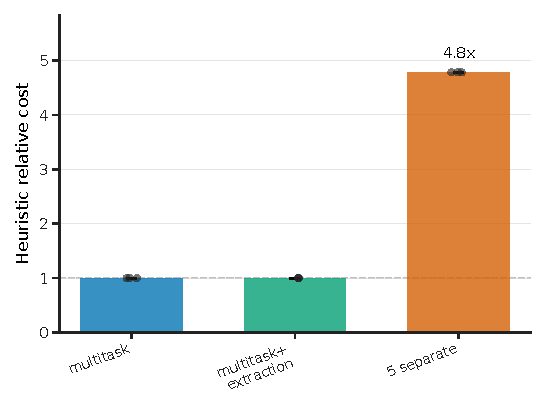
\includegraphics[width=90mm]{figs/supp_training_cost.pdf}
\caption{Auxiliary training and extraction accounting. Bars show means over three independent benchmark runs, error bars show s.e.m., and points show individual runs. The reference value of one is the jointly trained network plus extraction. The heuristic combines differently scaled proxies as specified in the text and excludes recomposition.}
\label{fig:training_cost}
\end{figure}

\end{document}
